\documentclass[11pt]{llncs}

\usepackage[english]{babel}
\usepackage[T1]{fontenc}
\usepackage[latin1]{inputenc}
\usepackage{times}
\usepackage{amssymb,amsmath,amscd,latexsym,graphicx}
\usepackage{tikz}
\usepackage{graphicx}
\usetikzlibrary{automata,positioning,calc,shapes.geometric}
\usepackage{framed}
%\usepackage[]{algorithm2e}
\usepackage{algorithm}
\usepackage[noend]{algpseudocode}
%\usepackage[usenames]{color}
\usepackage{fullpage}


\newcommand{\set}[1]{\{ #1 \}}
\newcommand{\N}{\mathbb{N}}
\newcommand{\A}{\mathcal{A}}
\newcommand{\M}{\mathcal{M}}
\newcommand{\perm}[1]{\langle #1 \rangle}
\newcommand{\ic}{\mathbf{ic}}
\newcommand{\e}{\mathbf{e}}
\newcommand{\re}{\mathbf{r}}
\newcommand{\val}[1]{\mathrm{val}(#1)}
\newcommand{\sem}[1]{[\![#1]\!]}
\newcommand{\New}{\mathbf{New}}


\newcommand{\trans}[1]{\stackrel{#1}{\longrightarrow}}
\newcommand{\PSPACE}{\mathrm{PSPACE}}

\def\mynote#1{{\sf $\dagger$ #1 $\dagger$}}

% Remove the author and date fields and the space associated with them
% from the definition of maketitle!
%\makeatletter
%\renewcommand{\@maketitle}{
%\newpage
% \null
% \vskip 2em%
% \begin{center}%
%  {\LARGE \@title \par}%
% \end{center}%
% \par} \makeatother

\title{Acme++: Optimizing Stabilization Monoid Computation for Probabilistic Automata and the Star-Height Problem}

%\author{Nathana\"el Fijalkow\inst{1,2} \and Hugo Gimbert\inst{3} \and Edon Kelmendi\inst{3} \and Denis Kuperberg\inst{4}}
%\institute{LIAFA, Paris 7, France \and University of Warsaw, Poland \and LaBRI, Bordeaux, France \and Onera, Toulouse, France}


\begin{document}

\begin{center}
{\large
Acme++: Optimizing Stabilization Monoid Computation for Probabilistic Automata and the Star-Height Problem}
\end{center}

\begin{abstract}
We present Acme++, a tool manipulating stabilization monoids.

Acme++ can solve three fundamental algorithmic problems.  First, compute
the star-height of a regular language, i.e. the minimal number of
nested Kleene stars needed for expressing the language with a regular expression. Second, decide boundedness and equivalence for regular cost functions. Third, decide whether a
probabilistic automaton has value 1, i.e. whether a probabilistic
automaton accept words with probability arbitrarily close to 1.

All three problems reduce to the computation of the stabilization monoid associated with an automaton,
which is a challenge since the monoid is exponentially larger than the automaton.
The compact data structures used in Acme++, together with optimizations and heuristics, allow this program to handle automata with
several hundreds of states. This radically improves upon the performance of AcmeML,
a previous version of the tool.
\end{abstract}


\section{Introduction}

Acme++ is a tool for deciding properties of some algebraic structures called stabilization monoids,
with two motivations in mind:
\begin{itemize}
\item compute the star height of a regular language of finite words,
\item decide whether a probabilistic automaton has value $1$.
\end{itemize}

\textbf{The Star-height problem.} The Star-height problem takes as input a regular language $L$ and an integer $h$ and decides whether there exists a regular expression for $L$ with at most $h$ nested Kleene stars.
The minimal $h$ having this property is called the star height of $L$. 
An excellent introduction about the Star-height problem is given in \cite{Kirsten05},
which mentions some of the important industrial applications as
speech recognition \cite{Mohri97}, database theory \cite{GT01}, and image compression \cite{CK93,KMT04}.
This problem was considered as one of the most difficult problems in the theory of recognizable languages
and it took 25 years before being solved by Hashiguchi \cite{Hashiguchi88}.
Implementing Hashiguchi algorithm is hopeless: the algorithm proceeds by enumeration of certain expressions
and has a terrible complexity \cite{LS02}.
It took another 22 years before an algorithm with a better algorithmic complexity was given by Kirsten in \cite{Kirsten05}. Kirsten algorithm is based on the transformation of the input automaton on finite words to 
a nested counter automaton with the following key property: the counter automaton is \emph{unbounded}
if and only if the star height of the regular language is less than $h$. To checks whether the
counter automaton is unbounded, Acme++ computes the associated stabilization monoid.

Acme++ aims at solving the Star-height problem for practical applications,
albeit the doubly exponential space complexity of Kirsten's algorithm is a challenge to tackle.


\textbf{The Value 1 problem.} Probabilistic automata are a versatile tool widely used in speech recognition as well as a modelling tool for the control of systems with partial observation or no observation.
Probabilistic automata are a natural extension on automata on finite words,
with probabilistic transitions, see \cite{Rabin63} for an introduction.

The Value 1 problem takes as input a probabilistic automaton on finite words and checks whether there are words accepted with probability arbitrarily close to $1$, see~\cite{FGO12} for an introduction.
The Value $1$ problem is a reformulation of a natural controller synthesis problem:
assume a blackbox finite state system with random events
is controlled by a blind controller which inputs actions to the blackbox
but has absolutely no feedback on the state of the system.
Then the synthesis of controllers with arbitraily high reliability is equivalent to solving the value $1$ problem.



\textbf{ Stabilization monoids.} Stabilization monoids are the key mathematical object needed to solve both the Star-Height and the Value 1 problems:
computing the starheight of a language can be done by computation of the stabilization monoid of
nested distance desert automata and deciding whether a leaktight probabilistic automaton has value $1$
reduces to the computation of the associated Markov monoid.

The Star-Height problem is related to the limitedness problem of nested distance automata.
A seminal paper by Simon \cite{Sim94} unifies several results using monoids of matrices, providing in particular a combinatorial tool called the forest factorization theorem. 
The first proof of the computability of the star height was given by Hashigushi and was very intricate.
Hopefully, Kirsten gave a much more elementary and clean algorithm:
a language has star-height at most $h$ if and only if the stabilization monoid of an associated nested desert automaton contains an \emph{unbounded witness}.
Desert automata are automata with ranked counters that can be either incremented and reset,
with the extra condition that if a counter is reset all counters of lower rank are reset as well.
Colcombet extended further the work of Kirsten introducing stabilization monoids and generalizing regular language theory into cost function theory, including algebraic and logical characterizations \cite{Colcombet09,CKL10,Kup14}. 
The algebraic techniques of Simon were adapted to solve the value $1$ problem for probabilistic automata:
a leaktight automaton has value $1$ if and only if its Markov monoid
contains a value $1$ witness~\cite{FGO12}.

\textbf{An efficient implementation.} Computing stabilization monoids of automata is challenging since the construction induces an exponential blowup, and the two decision problems we tackle are PSPACE-complete. In order to find unbounded and value $1$ witnesses in the stabilizaton monoids, Acme++
% incrementally
%
%computes the whole stabilization monoid, which is described by a set of matrices on a finite domain together with %rewrite rules. The algorithm 
apply iteratively the productand stabilization operators of the monoid in order to generate all elements of the monoid, represented by a minimal collection of matrices on finite domains, and a set of rewrite rules that define how the product and the stabilization operators act on elements.
Acme++ search particular elements in the monoid and stops as soon a witness is found. If no witness is found then the whole monoid is computed before the algorithm stops and outputs a negative answer.

To cope with large monoids, Acme++ uses compact data structures. In particular the matrices representing elements are not stored explicitely in memory: each vector appearing as a row or a column is stored at most once and matrices only store pointers to these rows and vertices. This way, Acme++ was able to generate monoids with more than fifty thousands elements and could handle the construction of stabilizaton monoid of automata with several hundreds of states.

The Starheight computation performed by Acme++ relies on an optimization from \cite{CL08sh}: the structure of Subset Automata, whose algebraic properties allow minimization. Moreover, the complexity of the algorithm is simply exponential because the input of Acme++ are restricted to deterministic automata, or non-deterministic automata for the complement language (dualized for uniformity of the input).

The tool ACME++ is open source and available from Github, details are given on the wepage
\url{http://www.liafa.univ-paris-diderot.fr/\textasciitilde nath/acme++.htm}.

\textbf{Related work.}
This approach using weighted automata was generalized and inspired the rich theory of regular cost functions \cite{Colcombet09}, which allows to solve other problems 
like the Star-height problem on finite trees~\cite{CL08sh}, as well as others problems related to regular languages and reducible to boundedness of automata with counters~\cite{CL08sh,CL08b,CKLB13}.




\section{Stabilization Monoids for $B$- and Probabilistic Automata}

The notion of stabilization monoids appears in two distinct contexts.
It has first been developed in the theory of regular cost functions,
introduced by Colcombet~\cite{Colcombet09,Colcombet13}.
The underlying ideas have then been transferred to the setting of probabilistic automata~\cite{FGO12}.

\subsection{Stabilization Monoids in the Theory of Regular Cost Functions}

At the heart of the theory of regular cost functions lies the equivalence between different formalisms:
a logical formalism, cost MSO, two automata model, $B$- and $S$-automata, and an algebraic counterpart, stabilization monoids.

Here we briefly describe the model of $B$-automata, and their transformations to stabilization monoid.
This automaton model generalizes the non-deterministic automata by adding a finite set of counters.
Instead of accepting or rejecting a word as a non-deterministic automaton does, 
a $B$-automaton associates an integer value to each input word.
Formally, a $B$-automaton is a tuple $\A = \perm{A,Q,\Gamma,I,F,\Delta}$, where $A$ is a finite alphabet, $Q$ is a finite set of states, 
$\Gamma$ is a finite set of counters, $I \subseteq Q$ is the set of initial states, $F \subseteq Q$ is the set of final states, 
and $\Delta \subseteq Q \times A \times \set{\ic,\e,\re}^\Gamma \times Q$ is the set of transitions.

A transition $(p,a,\tau,q)$ allows the automaton to go from state $p$ to state $q$ while reading letter $a$ and performing action $\tau(\gamma)$ on counter $\gamma$. 
Action $\ic$ increments the current counter value by $1$, $\e$ leaves the counter unchanged, and $\re$ resets the counter to $0$.

%A run of the automaton $\A$ on a word $w = a_1 a_2 \dots a_n$ is a sequence $\rho = q_0,\tau_1,q_1,\tau_2,\dots, \tau_n, q_n$ such that $q_0 \in I, q_n \in F$, 
%and for all $i \in [1,n]$, $(q_{i-1},a_i,\tau_i,q_i) \in \Delta$.
The value of a run is the maximal value assumed by any of the counters during the run.
The semantics of a $B$-automaton $\A$ is defined on a word $w$ by 
$\sem{\A}(w) = \inf\set{\val{\rho} \mid \rho\text{ is a run of } \A \text{ on } w}$.
In other words, the automaton uses the non determinism to minimize the value among all runs.
In particular, if $\A$ has no run on $w$, then $\sem{\A}(w) = \infty$.

%If $\A$ is a $B$-automaton, its semantics $\sem{\A}$ is usually viewed as a cost function, \textit{i.e.} exact values are ignored, 
%and just boundedness properties are considered. 
%Consequently, we say that two $B$-automata $\A_1$ and $\A_2$ are equivalent if $\sem{\A_1}$ and $\sem{\A_2}$ are bounded on the same sets of words.

The main decision problem in the theory of regular cost functions is the limitedness problem.
We say that a $B$-automaton $\A$ is \emph{limited} if there exists $N$ such that for all words $w$, if $\sem{\A}(w) < \infty$, then $\sem{\A}(w) < N$.

\vskip1em
One way to solve the limitedness problem is by computing the stabilization monoid.
It is a monoid of matrices over the semiring of sets of counter actions $\set{\ic,\e,\re,\omega}^\Gamma$.
There are two operations on matrices: a binary composition called product and a unary operation called stabilization.

The stabilization monoid of a $B$-automaton is the set of matrices containing the matrices corresponding to each letter,
and closed under the two operations, product and stabilization.
As shown in~\cite{Colcombet09,Colcombet13}, the stabilization monoid of a $B$-automaton $\A$ contains an unlimited witness
if and only if it is not limited,
implying a conceptually simple solution to the limitedness problem: compute the stabilization monoid
and check for the existence of unlimited witnesses.

An unlimited witness will be in the form of a $\sharp$-expression, generated by the grammar $e:=A|ee|e^\sharp$, for instance $a(ba^\sharp bba)^\sharp$. It describes the sequence of operations to perform in the monoid in order to reach the witness from the generators (the matrices associated with the alphabet), as well as how to build a sequence of words of unbounded value, by replacing $\sharp$ by $n$.

The notion of stabilization monoid can be abstracted, and any set equipped with these two laws (product and stabilization) and verifying certain axioms can be considered as a stabilization monoid, and can be used to recognize a cost function. In particular stabilization monoids can be minimized, which allows equivalence testing of regular cost functions.

%Following the celebrated success for the star-height problem, whose decidability has been established by
%reducing it to the limitedness problem of $B$-automata~\cite{Hashiguchi88,Kirsten05}, 
%several problems have been reduced to this problem.
%For instance, we implemented the solution of the finite power property:
%given a regular language $L \subseteq A^*$, does there exist $n \in \N$
%such that $L^* = L^ 0 + L^1 + \cdots + L^n$?
%We reduce this problem to a limitedness problem for $B$-automata, following \cite{Kirsten02}.

\subsection{Stabilization Monoids for Probabilistic Automata}

The notion of stabilization monoids also appeared for probabilistic automata, for the Markov Monoid Algorithm.
This algorithm was introduced in~\cite{FGO12} to partially solves the value $1$ problem: given a probabilistic automaton $\A$,
does there exist $(u_n)_{n \in \N}$ a sequence of words such that $\lim_n \mathbb{P}_\A(u_n) = 1$?

Although the value $1$ problem is undecidable, it has been shown that
the Markov Monoid Algorithm correctly determines whether a probabilistic automaton has value $1$
under the \textit{leaktight} restriction.
It has been recently shown that all classes of probabilistic automata for which the value $1$ problem has been shown decidable 
are included in the class of leaktight automata~\cite{FGKO14},
hence the Markov Monoid Algorithm is the \textit{most correct} algorithm known to (partially) solve the value $1$ problem.

As for the case of $B$-automata, the stabilization monoid of a probabilistic automaton
is the set of matrices containing the matrices corresponding to each letter,
and closed under the two operations, product and stabilization.

Note that the main point is that both the products and the stabilizations depend on which type of automata is considered,
$B$-automata or probabilistic automata. In particular the two frameworks do not seem to be reducible to each other at the level of automata, meaning there is no simple transformation from probabilistic automaton to $B$-automaton (or vice-versa) which preserves the stabilization monoid associated with the automaton.


\section{Computing the Stabilization Monoid of an Automaton}

We report here on our implementation of the following algorithmic task:
\begin{framed}
We are given as input:
\begin{itemize}
	\item A finite set of matrices $S$,
	\item A binary associative operation on matrices, the product, denoted $\cdot$,
	\item A unary operation on matrices, the stabilization, denoted $\sharp$.
\end{itemize}
The aim is to compute the closure of $S$ under product and stabilization,
called the stabilization monoid generated by $S$.
\end{framed}

Note that if we ignore the stabilization operation, this reduces to computing the monoid generated by a finite set of matrices.
It is well-known that this monoid can be exponential in the size of the matrices,
so the crucial aspect here is space optimization.
We describe two optimizations that allow to significantly reduce space consumption.

Recall that in our application, the initial set of matrices is given by matrices $M_a$ for $a \in A$, 
where $A$ is the finite alphabet of the automaton.
Hence we naturally associate to every element of the stabilization monoid a $\sharp$-expression:
$(M_a \cdot M_b^\sharp \cdot M_a)^\sharp$ is associated to $(a b^\sharp a)^\sharp$.
Many $\sharp$-expressions actually correspond to the same matrix: for instance, it may be that
$(M_a \cdot M_a \cdot M_b)^\sharp = M_a^\sharp$.

\vskip1em
%The algorithm saturates $S$, alternating between closure by product and closure by stabilization.
The first optimization consists in storing a set $R$ of rewriting rules between $\sharp$-expressions,
in order to reduce as much as possible the number of products and stabilizations.

A typical step in the algorithm is to construct a new $\sharp$-expression using newly constructed elements.
Before computing the corresponding matrix,
we check beforehand that this $\sharp$-expression cannot be reduced using the rewriting
rules known so far:
\begin{itemize}
	\item if it can be reduced, we avoid the costly computation of a product or a stabilization,
	\item it it cannot be reduced, then we compute the corresponding matrix, check whether it appeared
	already. If it did appear, then add a rewriting rule, otherwise add the matrix.
\end{itemize}
This means that the algorithm processes a lot of new $\sharp$-expressions,
and should be able to quickly detect if a $\sharp$-expression can be rewritten using the set $R$.
This task is performed very efficiently thanks to an optimized representation of $R$
using pointers and a Hashing table.

\vskip1em
The second optimization is about how matrices themselves are stored in memory.
%The three operations performed on matrices are product, stabilization and equality check.
Empirically, although the stabilization monoid may contain a lot of different matrices,
these matrices are very similar to each other.
In particular, if we consider the set of lines of these matrices, it is rather small compared to the number of matrices.
Hence the idea of storing lines in a table, and matrices as a set of pointers to the corresponding lines.
This simple idea turned out to be a game changer.

The algorithm is presented in Algorithm~\ref{algo}.
\RestyleAlgo{boxed}
\begin{algorithm}[ht]
\KwData{$S = \set{(M_a,a) \mid a \in A}$}
\KwResult{The stabilization monoid generated by $S$}
Initialization: 
$\New = S$ and $R = \emptyset$ set of rewriting rules\;

\While{$\New \neq \emptyset$}{

	// Closure by product\;
	$\New_T = \New$\;
	$\New = \emptyset$\;
	\For{$(M,m) \in \New_T$}{
		\For{$(N,n) \in S$}{
			\If{$m \cdot n$ is not reducible using $R$}{
				Compute $M \cdot N$\;
				\If{$(M \cdot N,w)$ is in $S$ for some $w$}{
					Add $m \cdot n \rightarrow w$ to $R$\;
				}\Else{
					Add $(M \cdot N,m \cdot n)$ to $\New_T$ and to $\New$\;
				}
			}
		}
	}
	\vskip1em
	// Closure by stabilization\;
	$\New_T = \New$\;
	\For{$(M,m) \in \New_T$}{	
		Compute $M^\sharp$\;
		\If{$(M^\sharp,w)$ is in $S$ for some $w$}{
			Add $m^\sharp \rightarrow w$ to $R$\;
		}\Else{
			Add $(M^\sharp,m^\sharp)$ to $\New$\;
		}
	}

	Add $\New$ to $S$\;	
}
\Return{S}\;
\caption{\label{algo}Computing the stabilization monoid}
\end{algorithm}


\section{Benchmarks}
We compared the running times of Acme++ and the previous
implementation AcmeML to justify this upgrade. We report the results
in this section.

For the benchmarks we randomly chose automata which produce larger
Markov monoids in order to observe the difference in performance
between the two versions. The point of comparison is the size of the
computed monoid rather than the number of states in the automaton,
since some large automata can indeed produce small monoids, and
vice-versa, some small automata can produce large monoids.

To this extent, for each state $s$ we pick a state $t$ with uniform
probability on the set of states and add a transition between $s$ and
$t$. After this we uniformly pick a number $p\in[0,1]$, and for all
other states $t'$ different from $t$, we add a transition between $s$
and $t'$ by flipping a $p$-biased coin.

The results have been plotted in Fig. \ref{bench1}. 

If for some sizes of the monoid in the x-axis there is no
corresponding point for the AcmeML implementation, it means that it
either timed out or had a stack overflow.

\begin{figure}[h!]
  \label{bench1}
  \begin{center}
    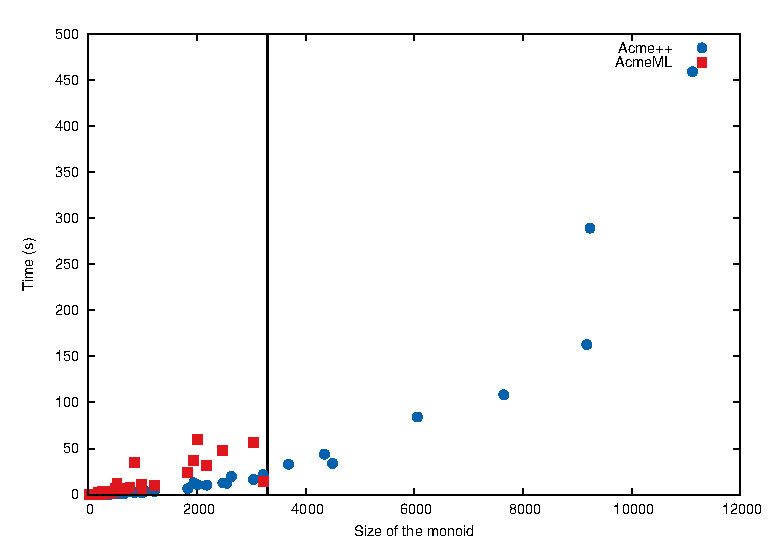
\includegraphics[width=0.8\textwidth]{graph/lines}
    \caption{The time it takes for the two implementations to
      calculate the Markov monoids generated by randomly picked
      automata of size 10}
  \end{center}  
\end{figure}

One can observe that there is a threshold in the size of the Markov
monoid after which AcmeML will not be useful. This threshold is
expressed by the vertical line in the graph above (it hovers around
3500 elements).

Even on smaller examples Acme++ outperforms AcmeML by a considerable
factor as seen in Fig. \ref{bench1zoomed}.

\begin{figure}[h!]
  \label{bench1zoomed}
  \begin{center}
    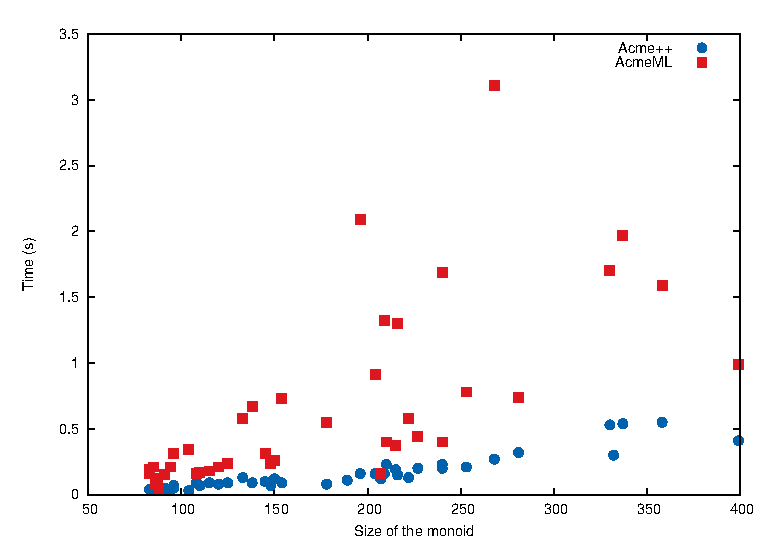
\includegraphics[width=0.8\textwidth]{graph/zoomlines}
    \caption{The same experiment as in Fig.\ref{bench1} on automata
      generating smaller Markov monoids}
  \end{center}  
\end{figure}



\newcommand{\cB}{\mathcal B}
% \newcommand{\trans}[1]{\stackrel{#1}{\longrightarrow}}

\section{The Star-Height algorithm}

The latest algorithm in the literature for computing star-height is designed for tree automata \cite{CL08sh}, but we will use it here in the special case of words. The main improvement over the previous algorithm from \cite{Kirsten05} is the identification of the structure of Subset Automata, which allows minimization.

We describe here briefly the ideas of the algorithm.

\subsection{Subset automata}

\begin{definition}\cite{CL08sh}
A subset automaton $\A$ is a deterministic automaton with additional $\epsilon$-transition, such that $\epsilon$-transition encode a lattice structure on the set space of $\A$. More precisely, $\epsilon$-transitions define a partial order on states, and for all states $p,q$, there are states $x,y$ such that $x\trans{\epsilon}p, x\trans{\epsilon}q, p\trans{\epsilon}y$ and $q\trans{\epsilon}y$.
\end{definition}

Due to the algebraic nature of their definition, subset automata can be minimized in a similar way to deterministic automata.

\begin{theorem}\cite{CL08sh}
Any language can be recognized by a subset automaton, obtained by a powerset construction from a non-deterministic automaton for the complement language.
\end{theorem}

\subsection{Reduction to limitedness}

Let $\A=\perm{A,Q,q_0,F_\A,\Delta_\A}$ be a subset automaton for a language $L$, and $k\in \mathbb N$. We recall that there are $\epsilon$-transitions, so $\Delta_\A\subseteq Q\times (A\cup\{epsilon\})\times Q$.

We build a $B$-automaton $\cB$ with $k+1$ counters $\gamma_0,\gamma_1,\dots,\gamma_k$, and states $Q_\cB=\bigcup_{i=1}^{k+1} Q^i$ that we view as a subset of $Q^*$.

Let $j\in[0,k]$, we will note $R_j$ the counter action performing $\re$ on counters $\gamma_p$ with $p\geq j$ and $\e$ on counters $\gamma_p$ with $p<j$. Simlarly, we will note $I_j$ the counter action performing $\re$ on counters $\gamma_p$ with $p> j$, $\ic$ on counter $\gamma_j$, and $\e$ on counters $\gamma_p$ with $p<j$. We finally note $\e$ the action performing $\e$ on all counters.
These particular counter actions are called \emph{hierarchical}, they correspond to the nested distance automata from \cite{Kirsten05}. Their advantage over general actions on multiple counters is that there is a total order or preference, namely $R_0\leq R_1\leq\dots R_k\leq \e\leq I_0\leq\ I_1\leq\dots\leq I_k$. This greatly simplifies the shape of elements of the stabilization monoid, since for each pair of states $(q_i,q_j)$ it suffices to store the best possible action to go from $q_i$ to $q_j$ instead of the set of all available actions.

The automaton $\cB$ is defined as follows:

\begin{itemize}
\item The initial state is $q_0$ (word of length $1$).
\item A state $wp$ is final if and only if $p\in F_\A$.
\item If $(p,a,q)\in\Delta$ and $w\in Q^{\leq k}$, there is a transition $wp\trans{a:I_{|w|}}wq$ in $\cB$. If $a=\epsilon$, the action may equivalently be equivalently replaced by $\e$, as we do in the implementation.
\item If $w\in Q^{\leq k-1}$ and $p\in Q_\A$, there is a transition $wp\trans{\epsilon:R_{|wp|}}wpp$ in $\cB$.
\item If $w\in Q^{\leq k-1}$ and $q,p\in Q_\A$, there is a transition $wpq\trans{\epsilon:R_{|wp|}}wq$ in $\cB$.
\end{itemize}


The following theorem guarantees the correctness of the reduction.
\begin{theorem}\cite{CL08sh}
The automaton $\cB$ is limited if and only if $L$ is expressible with a regular expression of star-height $k$.
\end{theorem}

Therefore, for any fixed $k$, we can decide in EXPSPACE whether a regular language has star-height $k$, if its is given via a nondeterministic automaton for the complement (or via a deterministic automaton).

The algorithm is as follow: build a subset automaton $\mathcal A$ via a powerset construction (exponential space), minimize it, then build the automaton $\cB$ as above, and finally test for limitedness of $\cB$ by building its stabilization monoid and looking for an unlimitedness witness.



\bibliographystyle{alpha}
\bibliography{bib}
\end{document}
